\section{Signalbeschreibung \skript{1}}
\subsection{Energie- und Leistungssignale \skript{3}}
\begin{tabular}{|l|l|l|}
	\hline
	\textbf{Klasse 1: Energiesignal} & \multicolumn{2}{|c|}{\textbf{Klasse 2: Leistungssignale}} \\
	\hline
	zeitbegrenzt oder abklingend,  	& \multicolumn{2}{|c|}{nicht zeitbregrenzt} \\ 
	einmalige Vorgänge, Impulse		& \multicolumn{2}{|c|}{}\\
	$W_n < \infty$		 	& \multicolumn{2}{|c|}{$W_n = \infty $} \\
	$P_n = 0$				& \multicolumn{2}{|c|}{$P_n \neq 0 $} \\
	\hline
							& \textbf{Klasse 2a: periodisch}	& \textbf{Klasse 2b: aperiodisch} \\
	\hline
	\parbox[c][4cm]{6cm}{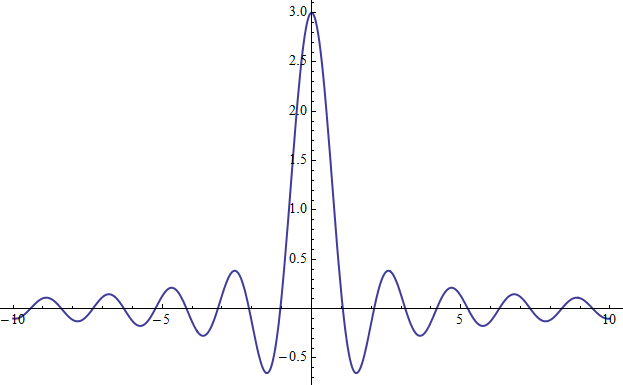
\includegraphics[width=5.9cm]{./bilder/Signale/SinusAbklingend.png}} &
	\parbox[c][4cm]{6cm}{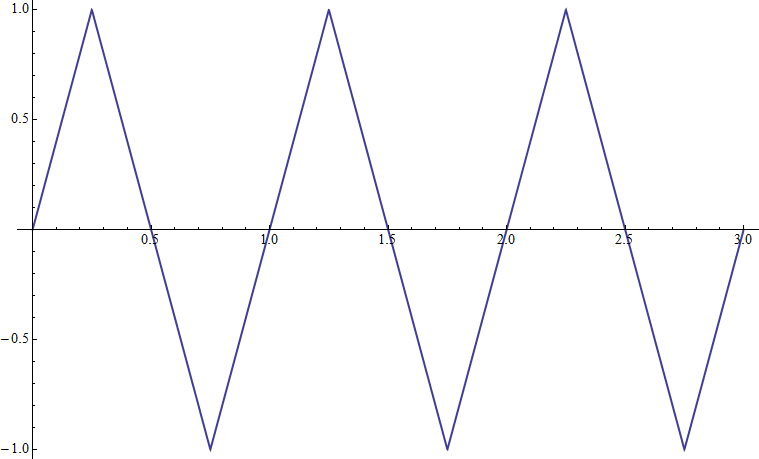
\includegraphics[width=5.9cm]{./bilder/Signale/Dreieck.png}} &
	\parbox[c][4cm]{6cm}{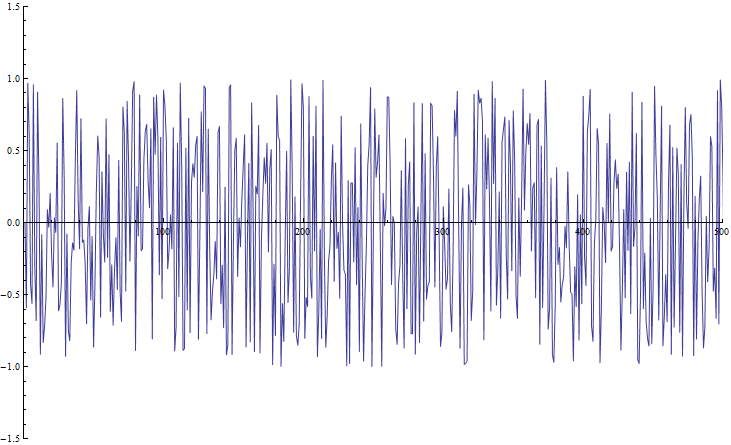
\includegraphics[width=5.9cm]{./bilder/Signale/Noise.png}} \\
	\hline
\end{tabular} \\

\begin{tabular}{|p{6cm}|p{6cm}|p{6cm}|}
 \hline
 	&\textbf{Zeitbereich} &  \textbf{Frequenzbereich} \\
 \hline
	 Normierte Signalenergie & $E_n = W_n =
	 \lim\limits_{T\to\infty}\,\int\limits_{-\frac{T}{2}}^\frac{T}{2}|f(t)|^2\,dt$ &
	 $E_n = \frac{1}{2\pi}\,\int\limits_{-\infty}^\infty|F(j\omega)|^2\,dt$ \\
 \hline
	 Normierte Signalleistung: & $P_n = \lim\limits_{T\to\infty}\,
	 \frac{1}{T}\int\limits_{-\frac{T}{2}}^\frac{T}{2}|f(t)|^2\,dt$ &  $P_n = \frac{1}{2\pi}\,\int\limits_{-\infty}^\infty\left(
	 \lim\limits_{T\to\infty}\frac{|F(j\omega)|^2}{T}\right)\,dt$ \\
\hline
\end{tabular}


\subsection{Mittelwerte \skript{5}}
\begin{tabular}{p{4.6cm}p{7.4cm}p{6cm}}
	Arithmetischer Mittelwert, Gleichwert, Linearer MW &
	$X_0 = \overline{X} = X_m = \frac {1} {T} \int\limits_{t_0}^{t_0+T} x(t)dt$ &
	(Kl. 2a) Ist die Fläche unter der Zeitfunktion über eine Periode.
    \\
	& $X_0 = \lim\limits_{T\to\infty} \frac{1}{T} \int\limits_{-\frac{T}{2}}^{\frac{T}{2}}x(t)dt \qquad$ &
	(Kl. 2b)\\	
		
	Quadratischer MW, Leistung &
	$X^2 = \frac {1} {T} \int\limits_{t_0}^{t_0+T} x^2(t)dt$ & 
	$X^n = \frac {1} {T} \int\limits_{t_0}^{t_0+T} x^n(t)dt$ (MW $n$. Ordnung) 
	\\
	Effektivwert &
	$X = X_{\text{eff}}= \sqrt{X^2} = \sqrt{\frac{1}{T} \int\limits ^{t_0+T} _{t_0}{x^2(t)dt}}$
	& 
	\\
	Gleichrichtwert &
	$X_{|m|} = \bar{|X|} = \frac{1}{T} \int\limits_{t_0}^{t_0+T}{|x(t)| dt}$ &
    Arithm. Mittelwert der Zweiweggleichrichterschaltung
    \\
	Varianz, Standardabweichung	&
	$\text{Var}(x)=\sigma^2= \frac {1} {T} \int\limits_{-T/2}^{T/2}(x(t)-X_0)^2dt = X^2-X_0^2$ &
	Mittl. Abweichung im Quadrat
	\\
	& $X^2 = var(x)+X_0^2 = |X|^2 = var(|x|) + |X_0|^2$ & \\
\end{tabular}

\newpage

\subsection{Funktionen}
\begin{tabular}{ll}
\textbf{Autokorrelationsfunktion (AKF)}
	& ``Wie weit wird die Zukunft von der Vergangenheit geprägt?'' \\
\parbox{6cm}{
	\skript{8}\\
	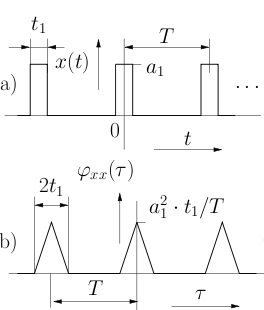
\includegraphics[width=4cm]{./bilder/akf1.png}\\
	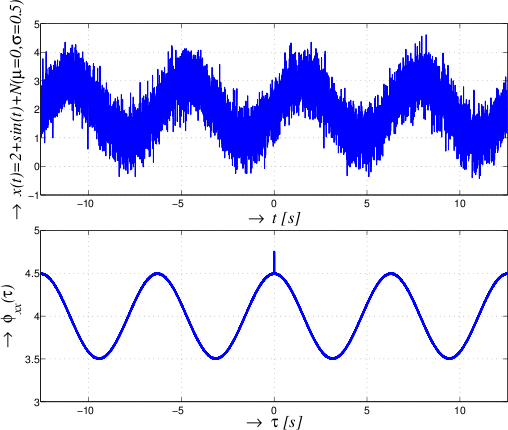
\includegraphics[width=4cm]{./bilder/akf2.png}
	} 
	& \parbox{12cm}{
	Für \textbf{Energiesignale} (Klasse 1):
	$$\varphi_{xx}(\tau) = \lim_{T\to\infty}\int\limits_{-T/2}^{T/2}
	x(t)x(t-\tau)dt=
	\lim_{T\to\infty}\int\limits_{-T/2}^{T/2} x(t+\tau)x(t)dt =
	\varphi_{xx}(-\tau)$$
	
	Für \textbf{periodische Leistungssignale} (Klasse 2a):
	$$\varphi_{xx}(\tau) = \frac {1} {T}
	\int\limits_{-T/2}^{T/2} x(t)x(t-\tau)dt 
	= \frac {1} {T} \int\limits_{-T/2}^{T/2} x(t+\tau)x(t)dt =
	\varphi_{xx}(-\tau)$$
	
	Für \textbf{nichtperiodische, stochastische Leistungssignale} (Klasse 2b):
	$$\varphi_{xx}(\tau) = \lim_{T\rightarrow\infty} \frac {1} {T}
	\int\limits_{-T/2}^{T/2} x(t)x(t-\tau)dt=\lim_{T\rightarrow\infty}\frac {1}
	{T} \int\limits_{-T/2}^{T/2} x(t+\tau)x(t)dt = \varphi_{xx}(-\tau)$$
	
	\textbf{Eigenschaften}
	\begin{itemize}
     \item $\varphi_{xx}(0) = X^2$ (Hat immer Diracstoss bei $\tau = 0$)
     \item $\varphi_{xx}(\tau)=\varphi_{xx}(\tau\pm mT)$, d.h. die
     AKF\index{Autokorrelationsfunktion} ist periodisch mit der gleichen Periode
     $T$ wie das Signal $x(t)$.
	\item $\varphi_{xx}(\tau)=\varphi_{xx}(-\tau)$: d.h. die AKF ist eine {\bf
	gerade Funktion}
	\item $\varphi_{xx}(0)\geq|\varphi_{xx}(\tau)|\quad$
	\item $\varphi_{xx}(\tau)\geq (X_0)^2-\sigma^2\quad$
   \end{itemize}
   \begin{tabular}{ll}
		 Beispiel: &$x(t) = a_k \cos(\omega t + \varphi) \Rightarrow \varphi_{xx}(\tau) =
		 \frac{a_k^2}{2} \cos(\omega \tau)$\\
		 & $x(t) = b_k \sin(\omega t + \varphi) \Rightarrow \varphi_{xx}(\tau) =
		 \frac{b_k^2}{2} \cos(\omega \tau)$ 
		\end{tabular}
	} \\
\hline & \\
\textbf{Kreuzkorrelationsfunktion (KKF)}
	& ``Wie ähnlich sind sich zwei Signale?'' \matlab{xcorr}\\
\parbox{6cm}{
 	\skript{11} \\
	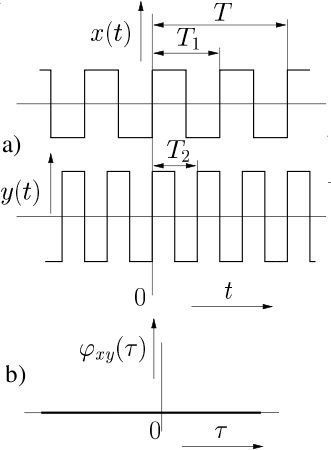
\includegraphics[width=4cm]{./bilder/kkf.png}
	}
	& \parbox{12cm}{
	Für \textbf{Energiesignale} (Klasse 1):
	$$\varphi_{xy}(\tau) = \lim_{T\rightarrow\infty}\int\limits_{-T/2}^{T/2}
	x(t)y(t-\tau)dt =\int\limits_{-T/2}^{T/2} x(t+\tau)y(t)dt$$ 

	Für \textbf{periodische Leistungssignale} (Klasse 2a):
	$$\varphi_{xy}(\tau) = \frac {1} {T} \int\limits_{-T/2}^{T/2}  x(t)y(t-\tau)dt
	= \frac {1} {T} \int\limits_{-T/2}^{T/2}  x(t+\tau)y(t)dt$$ 
		
	Für \textbf{nichtperiodische, stochastische Leistungssignale} (Klasse 2b):
	$$\varphi_{xy}(\tau) = \lim_{T\rightarrow\infty} \frac {1} {T}
	\int\limits_{-T/2}^{T/2}x(t)y(t-\tau)dt = \lim_{T\rightarrow\infty}\frac {1}
	{T} \int\limits_{-T/2}^{T/2} x(t+\tau)y(t)dt$$  
	
	Bei Signalen mit verschiedenen Frequenzen ist $\varphi_{xy}$ immer $0$, ausser die
	Gleichstromanteile!\\
	} \\
\end{tabular}

\begin{tabular}{ll}
\textbf{Sprungfunktion \skript{16}}
	& Einschaltfunktion, Einheitssprung, Heaviside-Function \matlab{heaviside} \\
\parbox{6cm}{
	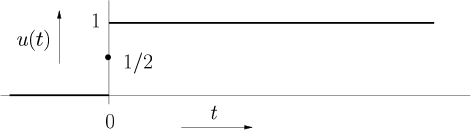
\includegraphics[width=5.5cm]{./bilder/sprungfunktion.png}
	}
	& \parbox{12cm}{
	$$u(t) = 1(t) = 
  \begin{cases}
    0 & \mbox{f"ur } t < 0,\\
    \frac{1}{2} & \mbox{f"ur } t = 0,\\
    1 & \mbox{f"ur } t > 0.\\
  \end{cases}$$	
	$$\mathcal{L:}\quad u(t) \laplace \frac1s$$
	} \\

\hline & \\
\textbf{Signumfunktion \skript{17}}
	& Vorzeichenfunktion \matlab{sign} \\
\parbox{6cm}{
	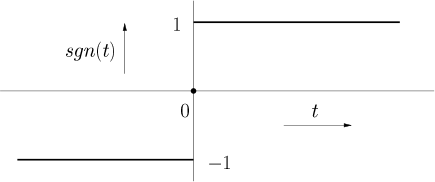
\includegraphics[width=5.5cm]{./bilder/sign.png}
	}
	
	& \parbox{12cm}{
	$$\sgn(t) =
  \begin{cases}
    -1 & \mbox{f"ur } t < 0,\\
    0 & \mbox{f"ur } t = 0,\\
    1 & \mbox{f"ur } t > 0.\\
  \end{cases}$$
	$$\mathcal{F:}\quad \sgn(t) \laplace \frac{-2j}{\omega}$$
	\\
	} \\
\hline & \\

\textbf{Rampenfunktion \skript{17}}
	& \matlab{ramp} \\
\parbox{6cm}{
	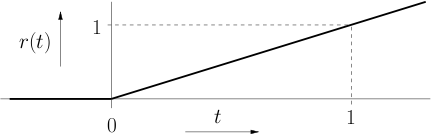
\includegraphics[width=5.5cm]{./bilder/ramp.png}
	}
	& \parbox{12cm}{
	$$r(t) = t u(t) =
  \begin{cases}
    0 & \mbox{f"ur } t \leq 0\\
    t & \mbox{f"ur } t > 0\\
  \end{cases}$$
	$$\mathcal{L:}\quad r(t) \laplace \frac{1}{s^2}$$
	\\
	} \\
\hline & \\

\textbf{Rechteckimpuls \skript{18}}
	&  \\
\parbox{6cm}{
	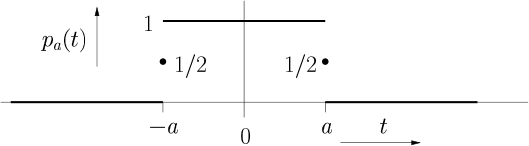
\includegraphics[width=5.5cm]{./bilder/rechteckimpuls.png}
	}
	& \parbox{12cm}{
	$$p_a(t) = u(t+a) -u(t-a) = 
  \begin{cases}
    1 & \mbox{f"ur } |t| < a\\
    \frac{1}{2} & \mbox{f"ur } |t| = a\\
    0 & \mbox{f"ur } |t| > a\\
  \end{cases}$$
	$$\mathcal{F:}\quad p_a(t) \laplace 2a \sinc(a \omega) = \frac{2}{\omega} \sin(a \omega)$$
	\\
	} \\
\hline & \\

\textbf{Dreieckimpuls \skript{19}}
	&  \\
\parbox{6cm}{
	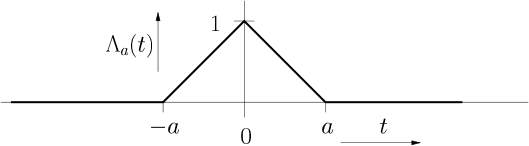
\includegraphics[width=5.5cm]{./bilder/dreieckimpuls.png}
	}
	& \parbox{12cm}{
	$$\Lambda_a(t) =
  \begin{cases}
    1 - \frac{|t|}{a}& \mbox{f"ur } |t| < a\\
    0 & \mbox{f"ur } |t| \geq a\\
  \end{cases}$$
	$$\mathcal{F:}\quad \Lambda_a(t) \laplace
	a\left(\frac{\sin(\frac{a\omega}{2})}{\frac{a\omega}{2}}\right)^2 = a \sinc^2\left(\frac{a\omega}{2}\right)$$ \\
	} \\
\hline & \\

\textbf{Sincfunktion \skript{19}}
	& \matlab{sinc}  \\
\parbox{6cm}{
	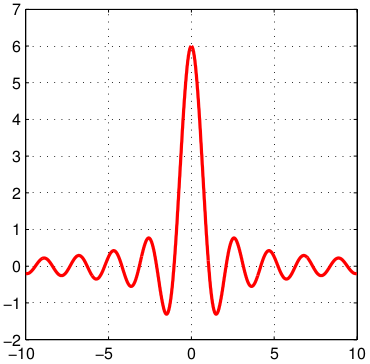
\includegraphics[width=5.5cm]{./bilder/sinc.png}
	}
	& \parbox{12cm}{
	$$ \sinc_{\alpha}(t) = \frac{\sin(\alpha t)}{t} \qquad 
	\sinc(\alpha t) = \frac{\sin(\alpha t)}{\alpha t}$$
	
	$$\mathcal{F:}\quad  \sinc_{\alpha}(t) = \frac{\sin(\alpha t)}{t} \laplace
	\pi p_{\alpha}(\omega)$$
	$$\mathcal{F:}\quad  \sinc(\alpha t) = \frac{\sin(\alpha t)}{\alpha t} \laplace
	\frac{\pi}{\alpha} p_{\alpha}(\omega)$$ } \\
\end{tabular}

\begin{tabular}{ll}
\textbf{Impulsfunktion \skript{20}}
	& Diracimpuls, Diracstoss, Deltaimpuls \matlab{dirac} \\
\parbox{5cm}{
	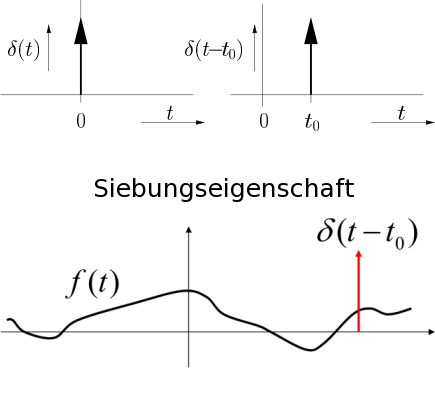
\includegraphics[width=5cm]{./bilder/dirac.png}
	}
	& \parbox{13cm}{
	$$\delta(t) =
  \begin{cases}
    \infty & \mbox{f"ur } t = 0\\
    0 & \mbox{sonst}\\
  \end{cases} \qquad \int\limits_{-\infty}^{\infty}\delta(t) dt = 1$$
	\begin{tabular}{|r|c|l|}\hline
	 1. & $\delta(at) = \frac{1}{|a|}\delta(t)$ & Skalierung\index{Skalierung}\\ \hline
	 2. & $\delta(\frac{t-t_0}{a}) = |a|\cdot\delta(t-t_0)$ & Skalierung und Verschiebung  \\ \hline
	 3. & $\delta(-t+t_0) = \delta(t-t_0)$ & symmetrisch\\ \hline
	 4. & $\delta(-t) = \delta(t)$ & $\delta(t)=\mbox{ gerade Funktion}$ \\ \hline
	 \textbf{5.} & $\int\limits_{-\infty}^{\infty}\delta(t-t_0)f(t)dt = f(t_0)$ & \textbf{Siebungseigenschaft}\\ \hline
	 6. & $\delta(t-t_0)f(t) = f(t_0)\delta(t-t_0)$ &  Abtastung\index{Abtastung}\\ \hline
	 \textbf{7.} & $\int\limits_{-\infty}^{\infty}A\cdot\delta(t)dt = A$ & \textbf{Spezialfall der Siebungseigenschaft} \\ \hline
	 8. & $\delta(t-t_0)\ast f(t) = f(t-t_0)$ & Faltung\\ \hline
	 9. & $\delta(t-t_1)\ast\delta(t-t_2) = \delta(t-t_1-t_2)$ & Faltung\index{Faltung}\\ \hline
	10. & $\int\limits_{-\infty}^t\delta(\tau)d\tau = u(t);	\qquad \delta(t)=\frac{\partial u(t)}{\partial t}$ & 
			Ableitung des Einheitssprungs\index{Ableitung}\\ \hline
	11. & $\delta(t)=\lim\limits_{\omega\rightarrow \infty}\frac{\sin(\omega
	t)}{\pi t}$ & Definition\\ \hline 
	12. & $\mathcal{L}, \mathcal{F}:\quad \delta(t) \laplace 1$ 
		& Frequenzbereich \\ 
	& $1 \laplace 2\pi\delta(\omega)$ & \\	
		\hline
	\end{tabular}\\
	\vspace{.1cm}\\
	} \\
\hline
\end{tabular}


\subsection{Rauschen \skript{24}}
\begin{tabular}{ll}
	& \matlab{randn} \\
\parbox{7cm}{
	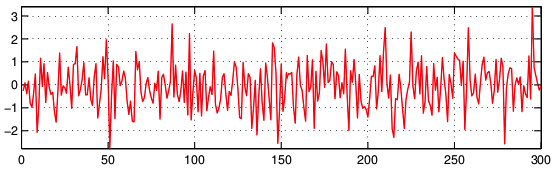
\includegraphics[width=7cm]{./bilder/rauschen.png}
	}
	& \parbox{11cm}{
	Ist die Intensit"at der
	Rauschspannung "uber viele Frequenzdekaden
	gleich verteilt, so spricht man von weissem Rauschen. \\
	Signal to Noise Ratio: $\text{SNR} =
	\frac{\text{Signalleistung}}{\text{Rauschleistung}}$ (rauschfrei $ \rightarrow
	\infty$) \\ 
	}
\end{tabular}

\begin{tabular}{lll}
	Signal-Rausch-Verh"altnis (SNR): &
	$a_r = 10\cdot \log_{10}(\frac{P_s}{P_r}) = 20\cdot \log_{10}(\frac{U_s}{U_r})$ &
	$P_s,U_s$: Nutzsignal\\
	
	Rauschzahl (noise figure): &
	$F = \frac{P_{sEingang}}{P_{rEingang}}\cdot\frac{P_{rAusgang}}{P_{sAusgang}}$ &
	$P_r, U_r$: Rauschsignal\\
	& $F=1$, bei einem idealen Vierpol &
	$T$: absolute Temperatur ($0^{\circ} = 273.15K$)\\
	
	Rauschmass: &
	$a_F = 10 \cdot \log_1(F) = a_{rEingang} - a_{rAusgang}$ & 
	$\Delta f$: Bandbreite\\
	
	Effektive Rauschspannung: &
	$U_r = \sqrt { 4 \cdot k \cdot T \cdot \Delta f \cdot R}$ & 
	$k = 1.380662\cdot 10^{-23}\frac{J}{K}$: Boltzmann-Konstante\\
	
	Effktive Rauschleistung: &
	$P_r = k \cdot T \cdot \Delta f$ & \\
\end{tabular}

\subsection{Amplitudenanalyse \skript{29}}
\begin{tabular}{ll}
	& ``Zeit während sich Signal in bestimmtem Amplitudenintervall aufhält'' \\
\parbox{7cm}{
	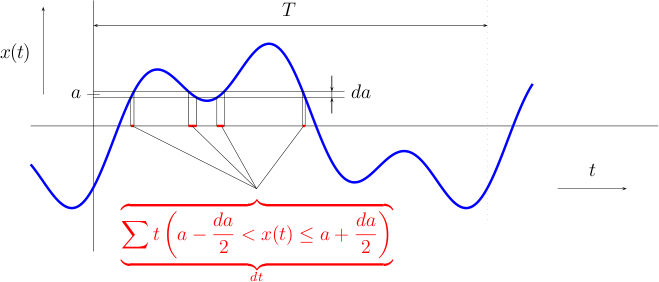
\includegraphics[width=7cm]{./bilder/amplitudenanalyse.png}
	}
	& \begin{minipage}[]{11cm}
			$$p(a) = \lim_{da\rightarrow 0}\frac{\underbrace{\sum t\left(
			a-\frac{da}{2}<x(t)\leq a+\frac{da}{2}\right)}_{dt}}{T\cdot da} = \frac{1}{T}\cdot
			\frac{dt}{da}$$
			$$\int\limits_{-\infty}^{\infty} p(a) da = 1; \qquad p(a) \geq 0  \quad \forall a$$
			
			\begin{tabular}{ll}
            Linearer Mittelwert 
            	& \fbox{$X_0  = \int\limits_{-\infty}^{\infty}a\cdot p(a)da$} \\ \\ 
            Mittelwert $n$. Ordnung 
            	& \fbox{$X^n = \int\limits_{-\infty}^{\infty}a^n\cdot p(a)da$} \\ \\
						Varianz
							& \fbox{$Var(x) = \int\limits_{-\infty}^{\infty}(a-X_0)^2\cdot p(a) da$} \\ \\
            \end{tabular}
      \end{minipage} \\
\end{tabular}

$\begin{array}{ll}
	x_1(t) \text{ mit} & p_1(a) \\
	x_2(t) \text{ mit} & p_2(a)
\end{array} 
\rightarrow x_3(t) = x_1(t) + x_2(t) \text{ mit } p_3(a) = (p_1 \ast p_2)(a)$

%\newpage

\begin{sidewaystable}
\begin{center}
\textbf{Zusammenstellung verschiedener Verteilungen \skript{39}} \\
\begin{tabular}{|c|c|c|c|c|}\hline
Verteilung & gleichverteilt & gaussf"ormig & sinusf"ormig & exponentiell\\ \hline\hline
 & 
	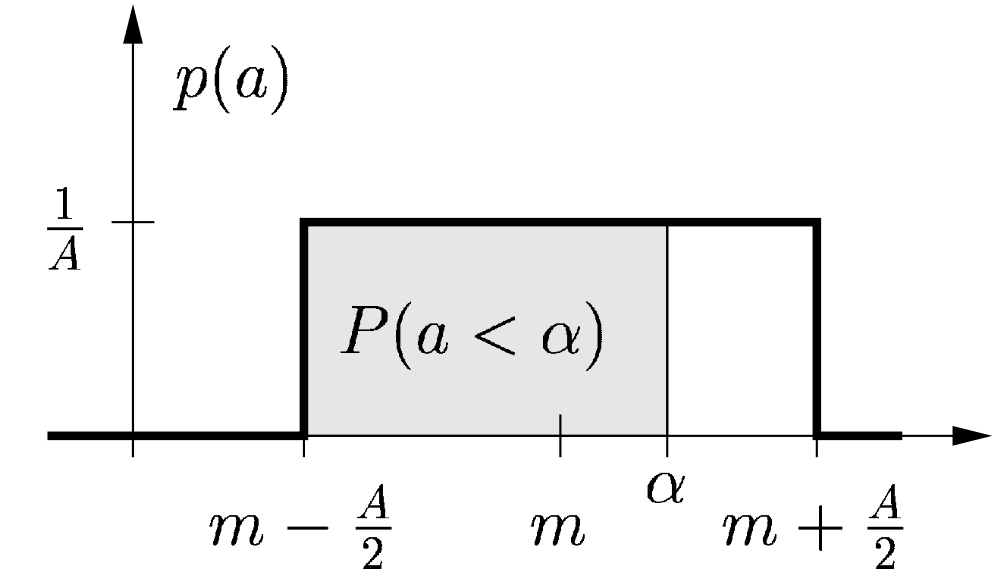
\includegraphics[width=4.3cm]{./bilder/verteilungen-gleichvert.png}
 &
	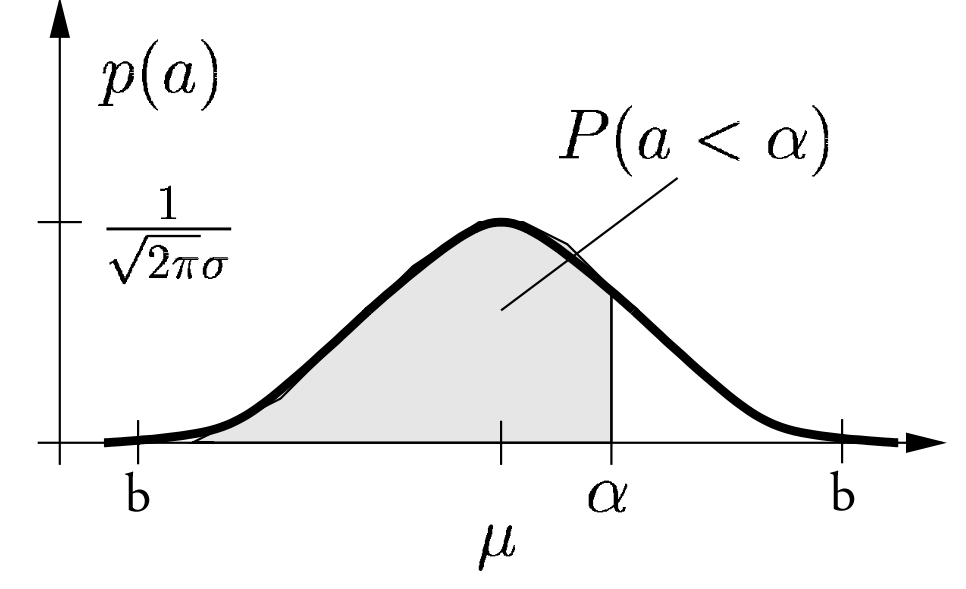
\includegraphics[width=4.3cm]{./bilder/verteilungen-gauss.png}
 &
	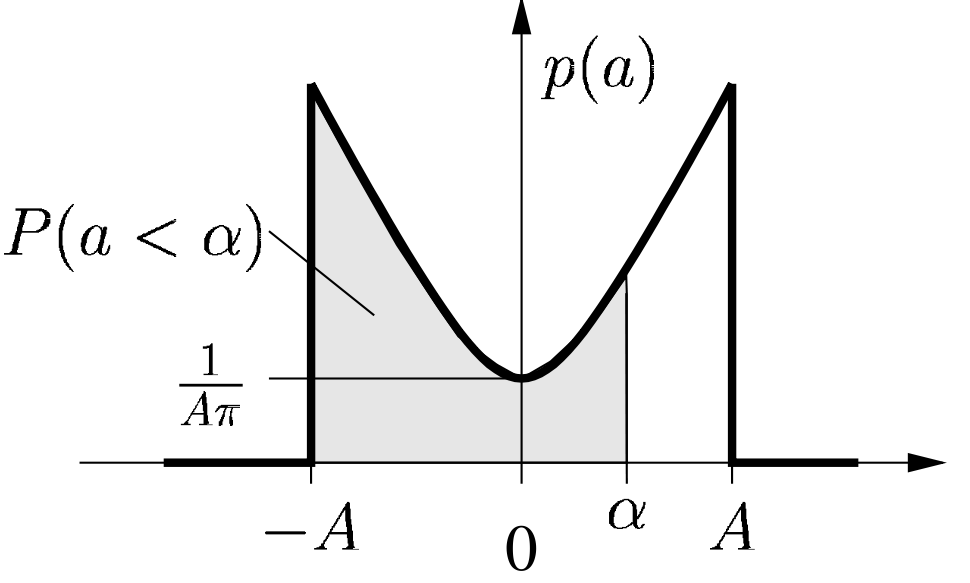
\includegraphics[width=4.3cm]{./bilder/verteilungen-sinus.png}
 &
	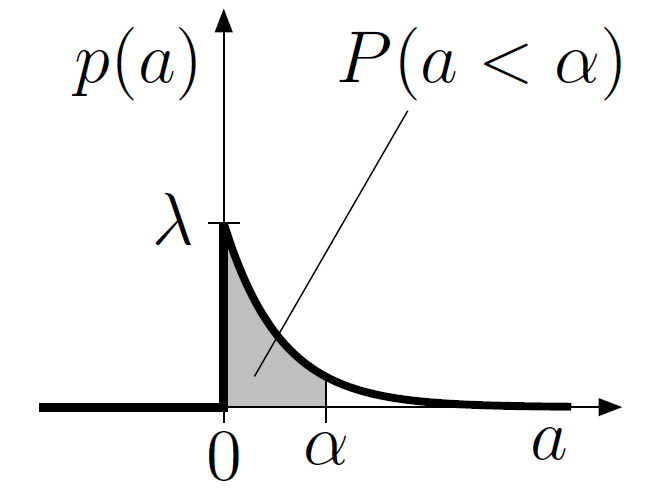
\includegraphics[width=4cm]{./bilder/verteilungen-expo.png} \\ \hline 
Amplitudendichte & & & & \\ $p(a)=$ & $\begin{cases} \frac{1}{A}&|a-m|\leq
\frac{A}{2},\\ 0&|a-m|>\frac{A}{2}.\\ \end{cases}$ &
$\displaystyle\frac{1}{\sqrt{2\pi}\sigma}e^{\displaystyle\frac{-(a-\mu)^2}{2\sigma^2}}$ & $\begin{cases} \frac{1}{\pi\sqrt{A^2-a^2}}&|a|\leq A,\\ 0&|a|>A.\\ \end{cases}$ &
 $\begin{cases} 
		\lambda e^{-\lambda a}  & a \geq 0\\
		0 & a < 0
	\end{cases}$\\ \hline  

 Wahrscheinlichkeit,& & & &\\ 
dass die Amplitude $a$ & & & &\\  
kleiner gleich $\alpha$ ist& & & & \\ 
$P(a\!\leq\!\alpha)\!=\!\!\int\limits_{-\infty}^{\alpha}\!p(a)da=$ &
$\begin{cases}0&\alpha<m-\frac{A}{2},\\ \frac{\alpha-(m-\frac{A}{2})}{A}&
|\alpha-m|\leq\frac{A}{2} \\1&\alpha\geq m+\frac{A}{2}. \end{cases}$  &
$Q\left(\frac{\displaystyle\mu-\alpha}{\displaystyle\sigma}\right)$ &
$\begin{cases}0&\alpha\!\leq\!-A,\\
\frac{1}{\pi}\left(\frac{\pi}{2}\!+\!\sin^{-1}\!\left(\frac{a}{A}\right)\right)&
|\alpha|\!<\!A,\\1&\alpha\geq A. \end{cases}$ &
$\begin{cases}
	0 & \alpha < 0\\
	1-e^{-\lambda \alpha} & \alpha \geq 0
\end{cases}$\\ \hline      
 & & & & \\ 
Mittelwert $X_0 =$& $m$ & $\mu$ & 0 & $\frac{1}{\lambda}$\\ 
& & & &\\ \hline
& & & &\\
Varianz $\operatorname{Var}(x) = $& $\dfrac{A^2}{12}$
& $\sigma^2$ & $\dfrac{A^2}{2}$ & $\frac{1}{\lambda^2}$\\ & & & & \\ \hline
& & & &\\
Leistung $X^2 =$& $m^2+\dfrac{A^2}{12}$ &
$\mu^2+\sigma^2$ & $\dfrac{A^2}{2}$ & $\frac{2}{\lambda^2}$ \\ 
& & & & \\ \hline
\end{tabular}

\textbf{Anmerkung zur gaussförmigen Verteilung:} Im Intervall $\mu \pm 3\sigma$
sind 99,73\% aller Messwerte zu finden. In der Zeichung ist diese Stelle mit
\textbf{b} gekennzeichnet.
\end{center}
\end{sidewaystable}




\newpage
\textbf{Zentraler Grenzwertsatz}\\ \\
	$X_1, X_2, \ldots , X_n$ sind lauter identisch verteilte (nicht notwendig normalverteilt!)
	unabhängige Zufallsvariablen mit demselben Erwartungswert $\mu$ und derselben Varianz $\sigma^2$
	und mit $Z = \frac{X-\mu}{\sigma}$\\
  Dann hat die Summe
	\begin{equation}
		S_n = \frac{1}{\sqrt{n}}\sum_{i=1}^n Z_i \nonumber
	\end{equation}
	den Erwartungswert $n \mu$ und die Varianz $n \sigma^2$. \\
  Die damit verbundene standardisierte ($E(S_n) = 0, var(S_n) = 1$) Variable $S_n$ ist somit wie
  folgt definiert: \\ 
	\begin{equation}
		S_n = \frac{1}{\sqrt{n}}\sum_{i=1}^n \frac{X_i - \mu}{\sigma}
		= \frac{1}{\sqrt{n}\cdot \sigma}\left[\left(\sum\limits_{i=1}^n X_i\right) -n \mu\right]
		=\dfrac{\bar{X} - \mu}{\sigma / \sqrt{n}} \nonumber
	\end{equation}
  Für $\boldsymbol{n \to \infty}$ strebt die Verteilung von $S_n$ gegen die
  Standardnormalverteilung. \\
\hrule

\begin{tabular}{ll}
\textbf{Faltung \skript{35}}
	& Convolution, ``Addition zweier unabhängiger ergodischer Prozesse $n_i$'' \matlab{conv} \\
\parbox{5cm}{
	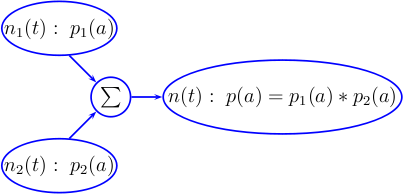
\includegraphics[width=5cm]{./bilder/faltung.png}
	\\}
	& \parbox{13cm}{
	$p(a) =
	\int\limits_{-\infty}^{\infty}p_1(\xi)\cdot p_2(a-\xi) d\xi = p_1(a)
	\ast p_2(a) =  p_2(a) \ast p_1(a) = \int\limits_{-\infty}^{\infty}p_2(\xi)\cdot 
  	p_1(a-\xi) d\xi$ \\
  	Die Breite des Faltungsproduktes entspricht der Summe der Breite der
  	einzelnen Faktoren.\\ \\
  	Faltung im Zeitbereich $\rightarrow$ Multiplikation im Frequenzbereich 
  	$$f(t) * g(t) \laplace F(s) G(s)$$
  	Faltung im Frequenzbereich $\rightarrow$ Multiplikation im Zeitbereich
  	$$F(s) * G(s) \Laplace \frac{1}{2 \pi} f(t) g(t)$$
		Faltung zweier Normalverteilungen
		$$N(\mu_1; \sigma_1) \ast N(\mu_2; \sigma_2) = N\left(\mu_1+\mu_2;\sqrt{\sigma_1^2+\sigma_2^2}\right)$$} \\
\end{tabular}

\begin{tabular}{ll}
\hline & \\
\textbf{Q-Funktion \skript{42}}
	& ``Wahrscheinlichkeit eines Fehlers'' \matlab{erf, erfc} \\
\parbox{6cm}{
	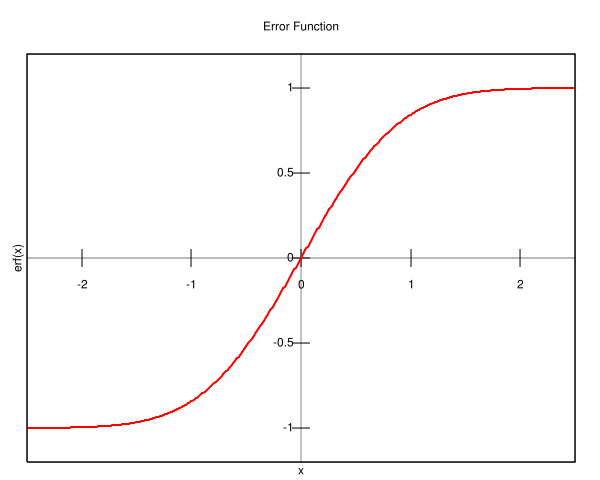
\includegraphics[width=5cm]{./bilder/q-funktion.png}
	}
	& \parbox{12cm}{
		Wenn die Resultate einer Messserie mit einer Normalverteilung mit Varianz
		$\sigma$ und Erwartungswert $0$ auftreten, dann ist
		$\operatorname{erf}\,\left(\,\frac{a}{\sigma \sqrt{2}}\,\right)$ die
		Wahrscheinlichkeit, dass ein einzelner Messwert zwischen $-a$ und $a$ liegt. 
		\\
		Tabelle \skript{53}\\
		$$Q(\xi)=\frac{1}{\sqrt{2\pi}}\int\limits_{\xi}^{\infty}
		e^{-\frac{y^2}{2}}dy$$
		$$Q(\xi) = \frac12 \operatorname{erfc}\left(\frac{\xi}{\sqrt2}\right)
		= \frac12 \left(1 - \operatorname{erf}\left( \frac{\xi}{\sqrt2}\right) \right)
		$$ }
\end{tabular}



